%!TEX program=xelatex
\documentclass[a4paper,10pt]{article}

\usepackage[linesnumbered,ruled,vlined]{algorithm2e}
\usepackage{amsmath}
\usepackage[backend=biber,style=alphabetic]{biblatex}
%\usepackage{ctex}
\usepackage[margin=16mm]{geometry}
\usepackage{graphicx}
\usepackage{hyperref}
\usepackage{indentfirst}
\usepackage{tikz}

\title{Borromean Ring Signatures}
\author{Sammy, Hao Xu}
\date{2017-09-21}

\addbibresource{REFERENCES.bib}
\hypersetup{
    colorlinks=true,
		citecolor=blue,
    linkcolor=blue,
    filecolor=magenta,      
    urlcolor=cyan,
}
\renewcommand{\vec}[1]{\mathbf{#1}}
% setting for algorithms
\SetKwProg{Fn}{}{}{}
\SetKwFunction{FnSigning}{Signing}
\SetKwInOut{Input}{input}
\SetKwInOut{Output}{output}
% end setting for algorithms
\usetikzlibrary{arrows,decorations.pathmorphing,positioning,fit,mindmap,petri}

\begin{document}
\maketitle

\section{Concrete Algorithm}
All the works listed in this section is from \cite{borromean-ring-signatures}.
\subsection{Signing}
Suppose a signer has a collection of verification keys $P_{i,j}$ for $0\leq i\leq n-1$, $0\leq j\leq m_i-1$, and wants to create a signature of knowledge of the $n$ keys $\{P_{i,j^*_i}\}_{i=0}^{n-1}$ where the $j^*_i$'s are some fixed and unknown (to a verifier) indices. Denote the secret key to $P_{i,j^*_i}$ by $x_i$. He acts as follows: 
\begin{enumerate}
	\item Compute $M$ as the hash of the message to be signed and the set of verification keys.
	\item For each $0\leq i\leq n-1$:
		\begin{enumerate}
			\item Choose a scalar $k_i$ uniformly at random.
			\item Set $L_{i,j^*} = k_iG$.
			\item For $j$ such that $j^*_i+1\leq j\leq m_i - 1$ choose $s_{i,j}$ at random and compute\label{comp1}
				\begin{eqnarray}
					e_{i,j} &= &H(M\| L_{i,j-1} \| i \| j - 1)	\\
					L_{i,j} &= &s_{i,j}G - e_{i,j}P_{i,j}
				\end{eqnarray}
		\end{enumerate}
	\item Finally, set 
			\[ 
				e_{i,0} = H(L_{0,m_0-1} \| \cdots \| L_{n-1,m_{n-1}-1}) 
			\] 
			That is, $e_{i,0}$ commits to several $(s, P)$ pairs, one from each ring.
	\item For each $0\leq i\leq n-1$:
		\begin{enumerate}
			\item Let \(L_{i,-1}=L_{i,m_i-1}\)
			\item For $j$ such that $0\leq j\leq j^*_i - 1$ choose $s_{i,j}$ at random and compute 
				\begin{eqnarray}
					L_{i,j} &= &s_{i,j}G-e_{i,j}P_{i,j} \\
					e_{i,j+1} &= &H(M\| L_{i,j}\|i\|j) 
				\end{eqnarray}
				Note that this calculation is identical to the one in Step $\ref{comp1}$.
			\item To wrap around making \(L_{i,j_i^*}=s_{i,j}G-e_{i,j_i^*}P_{i,j_i^*}\), we should set
				\begin{equation}
					s_{i,j_i^*}=k_i+x_i e_{i,j_i^*}
				\end{equation}
		\end{enumerate}
\end{enumerate}
The resulting signature on $m$ consists of
	\begin{equation}
		\sigma = \{ e_0, s_{i, j}\mid 0\leq i\leq n-1, 0\leq j\leq m_i - 1 \}
	\end{equation}
	where \(e_0\) means any of \(e_{i,0}\). We should publish 
	\begin{equation}
		\left\{M,\{P_{i,j}\},\sigma\mid 0\leq i\leq n-1, 0\leq j\leq m_i-1\right\}
	\end{equation}

\subsection{Verification}
Since verification does not depend on which specific keys are known, it avoids the ``two-phase'' structure of signing and is therefore much simpler.

We assume we have a message $m$, a collection $\{ P_{i,j} \}$ of verification keys whose indices range as before, and a signature $\sigma$ whose notation is the same as before. The verifier acts as follows:
\begin{enumerate}
	\item Compute $M$ as the hash of the message to be signed and the set of verification keys.
	\item For each $0\leq i\leq n -1$,
			\begin{enumerate}
				\item For each $0\leq j\leq m_i - 1$, compute 
					\begin{eqnarray}	
						L_{i,j} = s_{i,j}G - e_{i,j}P_{i,j} \\
						e_{i,j+1} = H(M\|L_{i,j}\|i\|j) 
					\end{eqnarray}	
					(As before, we always take $e_{i,0}$ to be $e_0$.)
			\end{enumerate}
	\item Compute 
			\begin{equation}
				e_0' = H(M\|L_{0,m_0-1} \|\cdots \| L_{n-1,m_{n-1}-1})
			\end{equation}
			and return 1 iff $e_0'\stackrel{?}{=} e_0$.
\end{enumerate}
A visualization of the whole scheme is as \figurename~\ref{fig-borromean-ring-sig}
\begin{figure}[!htbp]
	\centering
	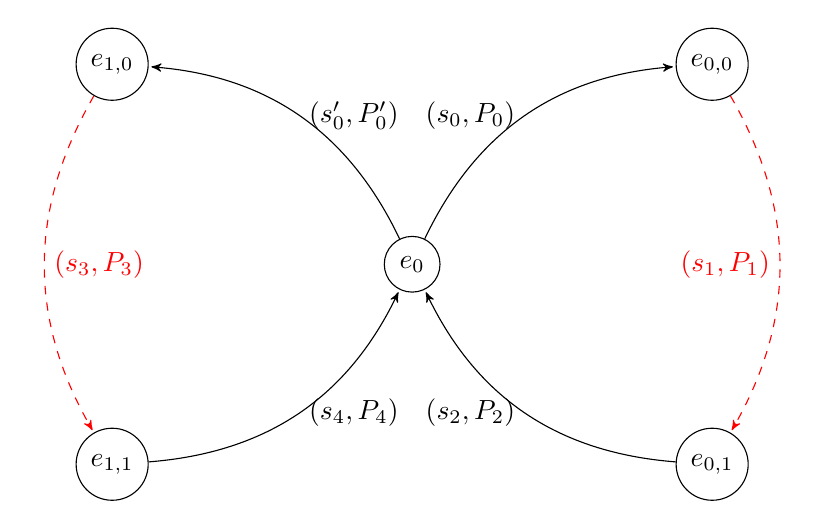
\begin{tikzpicture}[->,>=stealth',shorten >=1pt]
		\node[draw, circle] (e0) at (0in, 0in)     {$e_0$};
		\node[draw, circle] (e1) at (1.5in, 1in)   {$e_{0,0}$};
		\node[draw, circle] (e2) at (1.5in, -1in)  {$e_{0,1}$};
		\node[draw, circle] (e3) at (-1.5in, 1in)  {$e_{1,0}$};
		\node[draw, circle] (e4) at (-1.5in, -1in) {$e_{1,1}$};

		% left circle
		\path
			(e0) edge[bend right] node[right] {$(s_0', P_0')$} (e3)
			(e3) edge[bend right, dashed, color=red] node[right] {$(s_3, P_3)$} (e4)
			(e4) edge[bend right] node[right] {$(s_4, P_4)$} (e0);
		% right circle
		\path
			(e0) edge[bend left] node[left] {$(s_0, P_0)$} (e1)
			(e1) edge[bend left, dashed, color=red] node[left] {$(s_1, P_1)$} (e2)
			(e2) edge[bend left] node[left] {$(s_2, P_2)$} (e0);
	\end{tikzpicture}
	\caption{A Borromean ring signature for $(P_0 | P_1 | P_2) \& (P_0' | P_3 | P_4)$\label{fig-borromean-ring-sig}}
\end{figure}

\section{Implementation in Monero}
Summarized from the official codebase \cite{monero-project-codebase} as Algorithm~\ref{borromean-signing-in-monero} and ~\ref{borromean-verification-in-monero}, where \textcolor{red}{it commits on empty hash digest \(M\) and include no indices \( (i,j)\) in calculating \(e_{i,j}\)}.
\begin{algorithm}
	\DontPrintSemicolon
	\Input{\(\vec{x}\): set of secret keys \(\{x_i\}_{i=1}^{63}\)}
	\Input{\(\{\vec{P}_i\}\): set of pubkey rings, where \(\{\vec{P}_i=(P_{i,0},P_{i,1})\}\)}
	\Input{\(\{j_i^*\}\): indices set, s.t., for each pair \( (x_i,\vec{P}_i)\), \(P_{i,j_i^*}=x_i\cdot G\) for \(i=0,1,\dots,63\)}
	\Output{\(\sigma=(e_0,\{(s_{i,0},s_{i,1})\})\): \(e_0\) is a derived scalar, \(s_{i,0}, s_{i,1}\in_u R\)}
	
	\BlankLine
	\For{\(i\leftarrow 0\) \KwTo \(63\)}{
		\(k_i\in_u R\)\;
		\(L_{i,j_i^*}\leftarrow k_i\cdot G\)\;
		\If{\(j_i^*=0\)}{
			\(s_{i,1}\in_u R\)\;
			\(L_{i,1}\leftarrow s_{i,1}\cdot G+s_{i,1}\cdot P_{i,1}\)\;
		}
	}
	\(e_0\leftarrow H_s(L_{0,1}\|L_{1,1}\|\cdots\|L_{63,1})\)\;
	\For{\(i\leftarrow 0\) \KwTo \(63\)}{ 
		\eIf{\(j_i^*=0\)}{
			\(s_{i,0}=k_i-x_i\cdot e_0\)\;
		}{
			\(s_{i,0}\in_u R\)\;
			\(L_{i,0}\leftarrow s_{i,0}\cdot G+e_0\cdot P_{i,0}\)\;
			\(s_{i,1}\leftarrow k_i-x_i\cdot H_s(L_{i,0})\)\;
		}
	}
	\caption{The Implementation of Signing for Borromean Ring Signatures in Monero}\label{borromean-signing-in-monero}
\end{algorithm}
\begin{algorithm}
	\DontPrintSemicolon
	\Input{\(\{\vec{P}_i\}\), set of pubkey rings, where \(\{\vec{P}_i=(P_{i,0},P_{i,1})\}_{i=1}^{63}\)}
	\Input{\(\sigma=(e_0,\{(s_{i,0},s_{i,1})\})\), a signature generated by Algorithm~\ref{borromean-signing-in-monero}}
	\Output{true in case the verification is passed, and false otherwise}
	
	\BlankLine
	\For{\(i\leftarrow 0\) \KwTo \(63\)}{
		\(L_{i,0}\leftarrow s_{i,0}\cdot G+e_0\cdot P_{i,0}\)\;
		\(L_{i,1}\leftarrow s_{i,1}\cdot G+H_s(L_{i,0})\cdot P_{i,1}\)\;
	}
	\(\hat{e_0}\leftarrow H_s(L_{0,1}\|L_{1,1}\|\cdots\|L_{63,1})\)\;
	\Return \(\hat{e_0}=e_0\)\;
	\caption{The Implementation of Verification for Borromean Ring Signatures in Monero}\label{borromean-verification-in-monero}
\end{algorithm}
\printbibliography
\end{document}
